%-----------------------------------------------------
% Chapter: Background 
%-----------------------------------------------------
\chapter{Background}
\label{chap:background}
This chapter provides an introduction to the theory and previous work within the areas of word embeddings, neural language models and text classification. 

\section{Word Embeddings}
Word embeddings are vectors of predefined size which aim to encode a distributional numerical representation of word features. Recent aforementioned methods of learning these representations include the GloVe, word2Vec and fastText (\cite{Bojanowski2017}) algorithms. The utilization of word embeddings has been highly successful in many natural language processing tasks such as sentiment analysis (\cite{Socher2013}) and syntactic parsing (\cite{Socher2013}). Previous techniques for creating such representations can be categorised into two categories: matrix factorization methods and shallow window-based methods.
\subsection{Previous Methods}
\subsubsection{Global Matrix Factorization Methods}
Global matrix factorization methods such as Latent Semantic Analysis (LSA) use low rank approximations to decompose large matrices containing corpus statistics. Typically these matrices take the form of a term-document matrix, which captures the frequencies of terms across a collection of documents, or a term-term matrix, which store co-occurrence counts of terms. Matrix factorisation methods such as LSA allow for fast training and perform well on word similarity tasks by leveraging word occurrence statistics however they suffer from the disproportionate importance given to large word counts.
\subsubsection{Shallow Window-Based Methods}
Shallow window-based methods provide an alternative approach to learning word representations by sliding a fixed window over the contents of a corpus and learning to predict either the surroundings of a given word (skip-gram model) or predict a word given its surroundings (continuous bag of words). In the case of shallow window-based methods, they are good at capturing more complex patterns and do well in the word analogy task, however they fail to leverage global statistical information such as those used in global matrix factorization methods.
\subsection{GloVe}
Global Vectors for Word Representation (GloVe), is an unsupervised word embedding algorithm, introduced by Pennington et al, which marries the benefits of both global matrix factorisation and shallow window-based methods. Presented as a log-bilinear regression model, GloVe makes use of a global word co-occurrence statistics from a corpus. As detailed in the paper, GloVe outperformed previous methods such as word2vec in word analogy, word similarity and named entity recognition tasks. Conceptually, GloVe is based on the idea that ratios of probabilities of words co-occurring have the potential to encode meaning which is encoded as vector differences. This concept is formalised in the following equation, where the dot product of focal and context word vectors, \(w\) and \(\tilde{w}\), is equal to the logarithm of the probability of the words co-occurring, \(\log{X_{ij}}\).

\begin{equation}
w_{i}^{T} \tilde{w_{j}} + b_{i} + \tilde{b}_{j} = \log{X_{ij}}^{2}
\end{equation}

\noindent
\newline
A weighting function \(f(X_{ij})\) is used to decrease noise caused by very frequent word co-occurrences. The following weighting function is used in the GloVe model.

\begin{equation}
	f(x) =
	\begin{cases}
	(x/x_{max}), & \text{if  \(x <\) } x_{max} \\
	1, & \text{otherwise}
	\end{cases}
\end{equation}

\noindent
\newline
Combining equations 3.1 and 3.2, the GloVe model is defined as a weighted least squares regression problem.
\begin{equation}
	J = \sum_{i, j=1}^{N} f(X_{ij}) (w_{i}^{T} \tilde{w_{j}} + b_{i} + \tilde{b}_{j} - \log{X_{ij}})^{2}
\end{equation}
\subsection{CoVeR - Covariate-Specific Word Embeddings}
Covariates such as author demographics, time and location often accompany documents within a corpus. A trivial approach to obtaining covariate specific word embeddings involves applying GloVe to each subset of corpus documents mapping to a particular covariate. Unfortunately, utilising GloVe this way has certain drawbacks. Firstly, GloVe must be applied individually to sub corpora relating to a specific covariate, which, depending on the number of covariates, is time consuming. As a direct result of this, global co-occurrence statistics are now split into covariate specific co-occurrence statistics and these are not shared between embeddings, which may cause sub-optimal word representations, especially when sub corpora contain a small amount of co-occurrences for GloVe to leverage. 

\noindent
\newline
A known problem when representing words as dense representations using methods such as GloVe, is interpretability of dimensions. Due to conditional GloVe, producing word embeddings per corpora, relating these embeddings to one another becomes a difficult task. 


\noindent
\newline
Learning Covariate-Specific Vector Representations with Tensor Decompositions (CoVeR), proposed by Tian et al, provides an alternative to the conditional GloVe method which offers a framework to make learned embeddings more interpretable. Being an extension of GloVe, CoVer extends Glove's matrix decomposition of co-occurrence matrices to tensor decomposition of co-occurrence tensors, involving the joint learning of word embeddings and covariate specific transformation matrices which represent the effect of a particular covariate on the base embeddings learned. The CoVeR model is presented below.

\begin{equation}
J = \sum_{i, j=1}^{N} \sum_{k=1}^{M} f(X_{ijk}) ((c_{k} \odot w_{i})^{T} (c_{k} \odot \tilde{w}) + b_{ik} + \tilde{b}_{jk} - \log{X_{ijk}})^{2}
\end{equation}

\noindent
\newline
The introduction of covariate specific weight matrices into the objective function allows the authors to interpret dimensions in the base embeddings learned. 


\section{Language Models}
Formal languages such as programming languages are fully specified with precise syntax and semantics which dictate the usage of all reserved words within a language. Contrarily, natural languages, because of their emerging nature, are unable to be formally specified even with the existence of grammatical rules and structures. Unfortunately, rule based systems suffer from the endless possibilities of language usage outside of grammatical rules which are easily interpretable by humans. Moreover the task of consistently updating rule based systems to accommodate such usage is unfavourable.  

\noindent
\newline
Language modelling (LM) is the task of estimating the probability distribution of various linguistic units such as characters, words and sentences. In recent years, the application of LM  has been essential to many natural language process tasks such as speech to text and text summarization. Language models can be classified into two categories, count-based and continuous-space language models. 

\subsection{Count Based Models}
Count based methods such as statistical language models attempt to learn a probability distribution \(P(w_{1},...,w_{i}) \) over of a sequence of words \(w_{1},...,w_{i}\). An example of a count based method is the n-gram model.

\noindent
\newline
An n-gram is a sequence of \(n\) words. Examples of a two word sequences or bigrams include, \textit{"My name"} and \textit{"is Aubrey"}, whilst examples of three word sequences or trigrams, include sequences of words such as \textit{"Hello my name"} and \textit{"is Aubrey Graham"}. The n-gram model which considers the past \(n-1\) words can be formalised as 

\begin{equation}
	P(w_{i} | w_{1},...,w_{i-1}) \approx P(w_{i} | w_{i-n+1},...,w_{i-1})
\end{equation}

\noindent
\newline
The n-gram model relies on Markov assumptions to model the probability of word sequences \(P(w_{1}....w_{n}) \) as being equal to a limited number of previous words. An inherent problem with the n-gram model is sparsity as some word sequences occur rarely or not at all, even in large text corpora. Using the standard n-gram model would yield too many zero probabilities. To circumvent this, techniques such as back-off and smoothing exist. Another disadvantage of n-gram models is that they rely on exact patterns, meaning they fail to recognise syntactically and semantically similar sentences such as "the cat sat on the mat" and "the dog sat on the mat". N-gram models also suffer from the curse of dimensionality due to increased vocabulary sizes. As a result, limited window sizes are used, causing longer dependencies between words to not be captured.

\subsection{Neural Language Models}
To overcome issues faced by count based models, deep learning methods have been used to create neural language models by simultaneously learning word embeddings and the parameters needed to create a joint probability distribution between the word embeddings. \cite{Bengio2003} proposed a feed forward neural language model to help tackle the problem of data sparsity. Recent state of the art approaches such as \cite{Mikolov2010}, abstract language modelling as a form of sequential data prediction and have implored recurrent neural networks to help encode longer dependencies between sequences of words. The strength of these models comes from their ability to consider several preceding words and thus generalise well.

\noindent
\newline
An overview of generic neural network architectures as well as recurrent neural networks and Long-Short Memory networks are given in the following sections.

\subsubsection{Artificial Neural Networks}
In any neural network architecture, the elementary unit of computation is the artificial neuron which takes inspiration from biological neurons. The artificial neuron receives \(n\) inputs which are each weighted by \(n\) weights and summed together with a bias \(b\). The output \(y\) of a neuron is calculated by passing the weighted sum of the inputs into an activation function \(f\). 

\begin{equation}
	y = \left( \sum_{i=1}^{N} x_{i}w_{i} + b\right)
\end{equation}

\noindent
\newline
Typical activation functions include \textit{Sigmoid}, \textit{Tanh} and \textit{ReLu}. A single layer neural network is defined by \(k\) neurons sharing the same input in the same layer. Single layer neural networks have been proven to be \textit{'universal approximators'} (\cite{Hornik1989}) meaning any continuous function can be approximated using this type of network. The process of stacking layers on top of each other leads to multi-layer neural networks. These types of networks are also known as feed-forward networks. The learnable parameters of these networks are the set of weights and biases for each layer. A feed-forward neural network is trained using gradient descent and its parameters are updated using the \textit{backpropagation} algorithm (\cite{Rumelhart1988}).

\begin{figure}[h]
	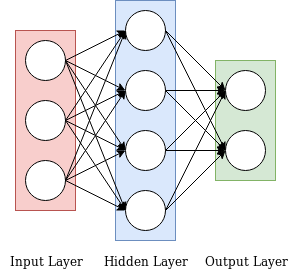
\includegraphics[width=8cm, height=8cm]{./figures/fig2}
	\centering
	\caption{Example neural network, three input nodes, four hidden and two outputs}
	\label{fig:fig2}
\end{figure}

\subsubsection{Recurrent Neural Network}
In a feed-forward neural network, data flow is unidirectional between layers; with data passing through a given neuron at most once. These types of networks perform well on both classification and regression tasks with the assumption that inputs are independent of each other. In tasks dealing with sequential data, feed-forward networks perform poorly. To model sequential data well, a neural network must be able to model the dependencies that exist between successive inputs. The recurrent neural network (RNN) is an attempt to satisfy this requirement by utilising past inputs to help predict future outputs.
\par
\noindent
\newline
In an RNN information is cycled within the network at least once.  An RNN receives a sequence of inputs \(x\) and updates its hidden state \(h_{t}\) by 

\begin{equation}
	h_{t}=
	\begin{cases}
	 0, & \text{t = 0} \\
	 \phi{(h_{t-1}, x_{t})}, & \text{otherwise}
	\end{cases}
\end{equation}

\noindent
where $\phi$ is a nonlinear function such as \textit{tanh} or \textit{ReLu}. The update for the hidden state is usually implemented as 

\begin{equation}
h_{t} = \phi{(Ux_{t} + Wh_{t-1})}
\end{equation}

\noindent
where W and U are weight matrices.

\par
\noindent
\newline
RNN's are trained using gradient descent and backpropagation through time (BBTT), which is identical to performing backpropagation on an \textit{"unrolled"} RNN (seen in figure \autoref{fig:fig3})

\begin{figure}[h]
	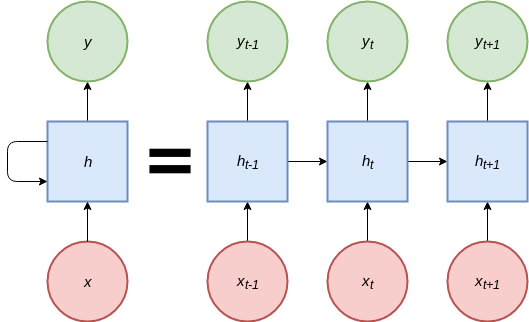
\includegraphics[width=10cm, height=6cm]{./figures/fig3}
	\centering
	\caption{An \textit{unrolled} recurrent neural network can be seen as a feed-forward neural network with many hidden layers}
	\label{fig:fig3}
\end{figure}

\par
\noindent
\newline
During BBTT, back propagation is performed on an unrolled recurrent architecture, causing gradients to back-propagate through numerous network layers. Unfortunately, this has a few major problems. Firstly, a single forward/backward pass through the network is computationally expensive due to the number of hidden layers of the unrolled network being linear to the number of time steps in a sequence. Secondly, this method suffers from the issue of vanishing or exploding gradients(REF) where gradients can decay or grow exponentially as they propagate over time, which can prevent the network from learning entirely.

\subsubsection{Long Short-Term Memory}
Long Short-Term Memory (LSTM) (\cite{Hochreiter1997}) is a variant of the recurrent neural network which is capable of capturing longer dependencies between sequences of data without suffering from vanishing gradients. This is achieved through a feature known as gating; a mechanism which acts as a permissive or restrictive barrier to information flow. 

\noindent
\newline
The core component of the LSTM is the cell state which is able to propagate \textbf{relevant} information throughout the network. This is achieved within the memory cell through the forget, input and output gate. The forget gate regulates how much of the existing memory should be forgotten, the input gate regulates how much of the new cell state to keep, and the output gate regulates how much of the cell state should be allowed into the next layer of the network.

\begin{figure}[h]
	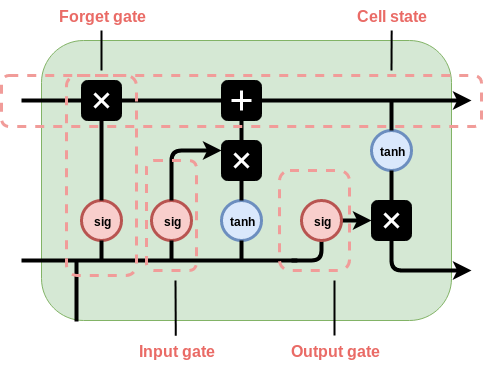
\includegraphics[width=10cm, height=8cm]{./figures/fig4}
	\centering
	\caption{LSTM memory cell, with forget, input and output gates}
	\label{fig:fig4}
\end{figure}

\subsection{Text Classification}
Text classification is a supervised NLP task which involves assigning pre-defined labels to text according to its content. Automated classification of text can be achieved through rule based and machine learning based systems. Rule based methods tackle classification through the use of handcrafted linguistic rules, which assign patterns in text to predefined categories. For example, given two word lists which  Rule based systems don't come without drawbacks, firstly to create such a system requires deep domain knowledge. Moreover, unlike the previous example, creating, maintaining and scaling such rules is challenging and time consuming. 
\subsubsection{Traditional Methods}
Before a classifier can be trained, textual inputs must be transformed into numerical representations in a process known as feature extraction. A common method for feature extraction is the bag of words approach which given a vocabulary set \(V\), creates an input vector which represents word counts for each word of the vocabulary. For example, if we define the vocabulary \(V\) ..

\noindent
\newline
Two common classifiers, namely Naive Bayes classifiers and support vector machines are outlined below

\paragraph{Naive Bayes}
\noindent
\newline 
Naive Bayes Classification is a generative approach which uses bayes theorom to learn a join probability distribution .... Naive bayes classification is a robust method for training a text classifier which can achieve accurate results without large amounts of training data.

Naive bayes is a classification techinque based on bayes theroem with an assumpoion of inde[endence among preictors. A naives bayes c;assifier assumes that the precence of a particular fgeature in a class is unrelsted tp the [recence of any other fetaure.

\paragraph{Support Vector Machines}
\noindent
\newline 
A Support Vector Machines (SVM) (Vapnik et al 1995) is a discriminative classifier that aims to find a linear classification boundary or \textit{hyperplane} to discriminate between classes in high dimensional space. SVM's achieve this through support vectors, random training data points, which are used to maximise the margin between ... Similar to naive bayes classifiers, SVM's do not require large amounts of training data to achieve accurate results. SVM's were introduced to the problem of text classification by Joachims(REF)

\subsubsection{Deep Learning Methods}